\documentclass[tikz,border=2pt]{standalone}
\usepackage{amsmath,amssymb}
\usepackage{tikz}
\usetikzlibrary{arrows.meta}

\begin{document}
% A homogeneous system Ax = 0 always has the trivial solution and its solution set is a
% subspace (here a line through 0); the inhomogeneous system Ax = b is a shifted copy.
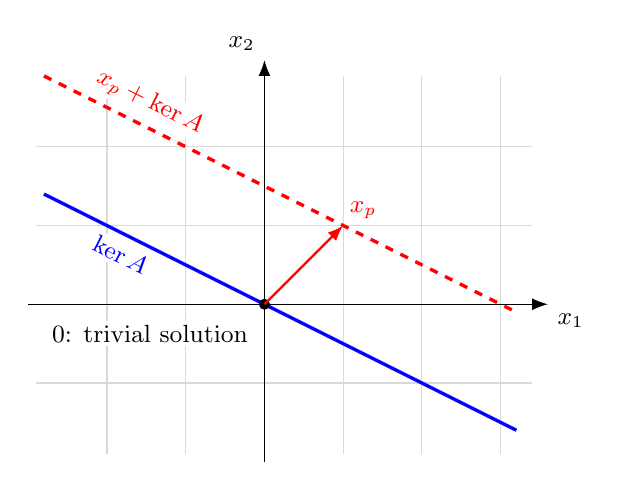
\begin{tikzpicture}[every node/.style={font=\small}, >={Latex[length=2mm]}]
	\draw[gray!30, step=1] (-2.9,-1.9) grid (3.4,2.9);
	\draw[->] (-3,0) -- (3.6,0) node[below right] {$x_1$};
	\draw[->] (0,-2) -- (0,3.1) node[above left] {$x_2$};
	\draw[blue, very thick] (-2.8,1.4) -- (3.2,-1.6);
	\node[blue, font=\small, rotate=-26.57, anchor=north, fill=white, inner sep=1.5pt] at (-1.75,0.78) {$\ker A$};
	\draw[red, very thick, dashed] (-2.8,2.9) -- (3.2,-0.1);
	\node[red, font=\small, rotate=-26.57, anchor=south, fill=white, inner sep=1.5pt] at (-1.55,2.38) {$x_p+\ker A$};
	\fill (0,0) circle (2pt);
	\node[anchor=north east, font=\small, fill=white, inner sep=1.5pt] at (-0.15,-0.2) {$0$: trivial solution};
	\draw[->, red, thick] (0,0) -- (1,1) node[above right, inner sep=2pt, font=\small] {$x_p$};
\end{tikzpicture}
\end{document}
